\subsection{Übertragung eines Lichtsignals} % (fold)
\label{sub:Übertragung eines Lichtsignals}
\begin{frame}
    \frametitle{Übertragung eines Lichtsignals}
    \framesubtitle{}
     \begin{columns}[c]
         \column{0.6\textwidth}
        \begin{block}{Ziel:}
             \begin{itemize}
                 \item Filterung der Störungen durch
                 \begin{itemize}
                     \item Lampen
                     \item Tageslicht
                 \end{itemize}
             \end{itemize}
        \end{block}
        \begin{block}{Versuch}
            \begin{itemize}
                \item moduliere LED-Signal mit $777Hz$ Spannung
                \item gebe Modulationsfrequenz als Referenzfrequenz weiter
                \item benutze L-I-Verstärker um $777Hz$ herauszufiltern
            \end{itemize}
        \end{block}
         \column{0.4\textwidth}
         \begin{figure}[H]
         \begin{center}
                 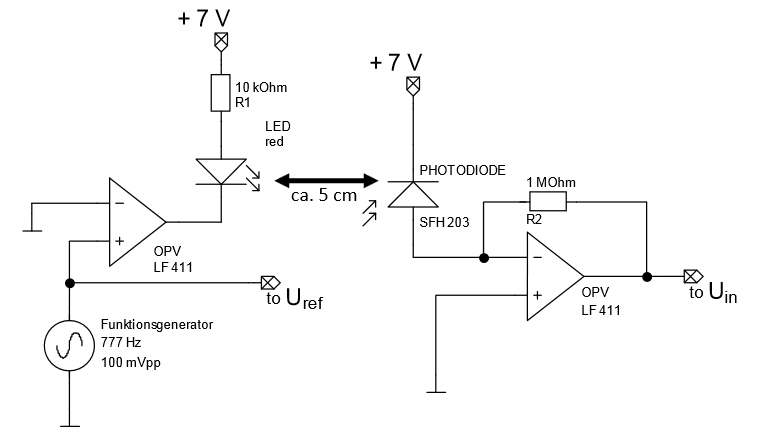
\includegraphics[scale=0.25]{./img/schaltung/optisch.png}
         \end{center}
         \end{figure}
     \end{columns}
\end{frame}

\begin{frame}
    \frametitle{Vergleich mit/ohne Abdeckung}
    \framesubtitle{}
    \begin{columns}[c]
        \column{0.5\textwidth}
        \begin{figure}[H]
        \begin{center}
                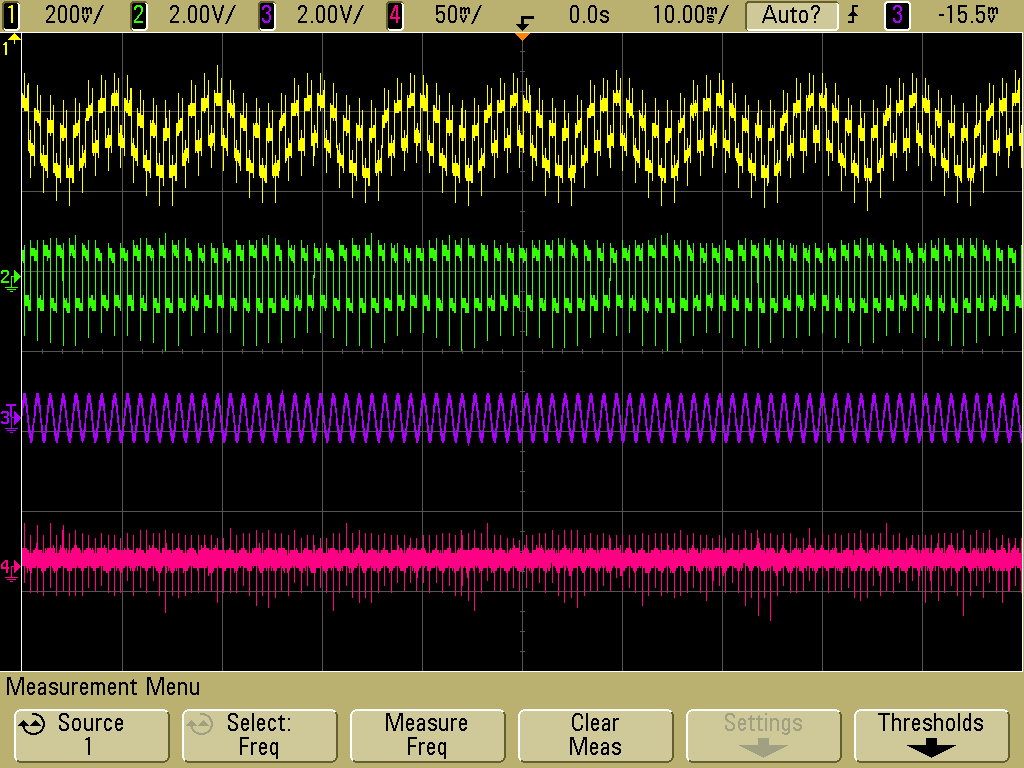
\includegraphics[scale=0.15]{./img/oszi/scope_23.png}
        \end{center}
        \caption{Ohne Abdeckung}
        \end{figure}
        \column{0.5\textwidth}
        \begin{figure}[H]
        \begin{center}
                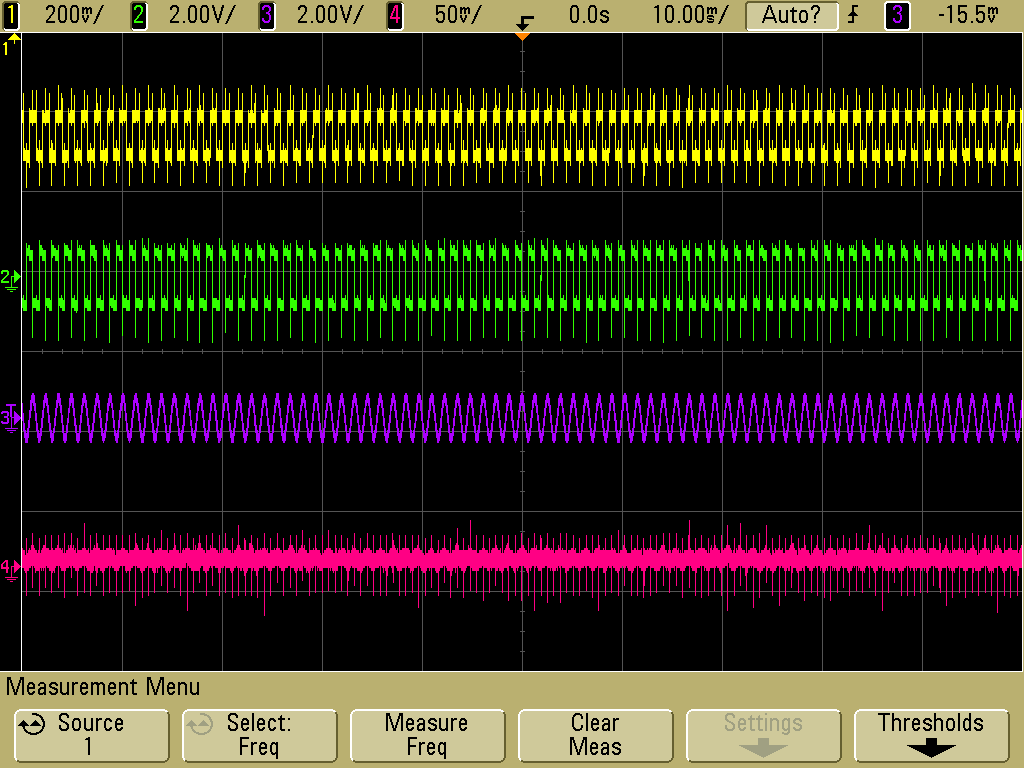
\includegraphics[scale=0.15]{./img/oszi/scope_22.png}
        \end{center}
        \caption{Mit Abdeckung}
        \end{figure}
    \end{columns}
        \begin{block}{}
            Ausgangssignal bleibt konstant auf $52.6mV$ $\rightarrow$ Schaltung
            filtert Störsignale heraus
        \end{block}
\end{frame}
% subsection Übertragung eines Lichtsignals (end)
